\documentclass{article}

\textwidth=6.5in
\textheight=8.5in
\voffset=-54pt
\oddsidemargin=0in
\evensidemargin=0in
\setlength{\parskip}{8pt}
\setlength{\parindent}{0pt}

\usepackage{workbook}

\usepackage{handout}

\usepackage{exam}

\newcommand{\answerbox}[3][]{
    \fbox{\begin{minipage}[t][#2][c]{#3}
        #1
    \end{minipage}}
    }

\begin{document}

{\large \mbox{} \hfill \bf Name:\underline{\hspace{3in}}}\\[2pt]
{\mbox{} \hfill \it (Please write your name neatly in print.)}\\[12pt]
{\large \mbox{} \hfill \bf HUID:\underline{\hspace{3in}}}
 
\medskip
 
\noindent
{\large\bf
Final Exam Practice 1\\
Math Mb Spring 2025}
\noindent


{\Large
\begin{center}\textbf{Directions---Please read carefully!} \end{center}}

This is a practice test. The same directions will appear on the actual exam, so read them carefully.

\hrulefill 


This exam is subject to the Harvard College Honor Code. No calculators or any other aids are permitted.  Please write as neatly as possible, as answers that can't be read can't be graded and thus can't receive credit. To receive full credit, you must show relevant working
and include units when appropriate. 

You have 180 minutes to complete this exam. 

You may ask for scratch paper if you need additional space to write, but it will not be scanned or graded. Make sure to include all relevant working in this exam booklet in the space provided for each question.

\begin{center}\textbf{Good luck!}\end{center}


\vfill

\centering{
\emph{As a member of Harvard College, I pledge that I will not give or receive assistance on this exam.}}
\vspace{0.3in}

{\large \mbox{} \hfill \bf Signature:\underline{\hspace{3in}}}
\thispagestyle{empty}

\newpage

\begin{enumerate}

  \item \label{Problem1-2023Final}
  
  Compute the following integrals and limits. \textbf{Simplify your answers wherever possible.} 
  

  \begin{enumerate}
      \item $\displaystyle \int_0^{\pi/2} 3\cos(x)\;dx$
      
      \begin{solution}
          \begin{align*}
          \displaystyle \int_0^{\pi/2} 3\cos(x)\;dx &=  3 \sin x \Big|_0^{\pi/2} \\
          &= 3\sin(\dfrac{\pi}{2})-3\sin(0)\\
          &= 3(1)-3(0)\\
          &= \boxed{3}
      \end{align*}
      \end{solution}

      \vfill
      
      \item $\displaystyle \int_0^1 \dfrac{10}{1+x^2}\, dx$

      \begin{solution}
      \begin{align*}
          \displaystyle \int_0^1 \dfrac{10}{1+x^2}\, dx &= 10\arctan x \Big|_0^1\\
          &= 10\arctan1-10\arctan0\\
          &= 10\left(\dfrac{\pi}{4}\right)-10(0)\\
        &= \boxed{\dfrac{10\pi}{4}}
      \end{align*}
      \end{solution}
      \vfill
      \item $ \displaystyle \int_0^1 \dfrac{x}{x^2+1}\, dx$
      
      \begin{solution}
          Let $u=x^2+1$. Then $du=2x\,dx$, so $\dfrac{1}{2}du = xdx$. Our new lower bound is $u=0^2+1=1$ and out new upper bound is $u=1^2+1=2$.
          \begin{align*}
              \displaystyle \int_0^1 \dfrac{x}{x^2+1}\, dx &= \displaystyle \int_1^2 \dfrac{1}{u} \cdot \dfrac{1}{2} \, du\\
              &= \dfrac{1}{2}\ln|u| \Big|_1^2\\
              &= \dfrac{1}{2}\ln|2|-\dfrac{1}{2}\ln|1|\\
              &= \boxed{\dfrac{1}{2}\ln 2}
          \end{align*}
      \end{solution}
      \vfill
      \pagebreak
      \item $\displaystyle \int 5\sin^2(x)\cos(x)\, dx$

      \begin{solution}
          Let $u=\sin x$. Then $du = \cos x\, dx$. So,
          \begin{align*}
              \displaystyle \int 5\sin^2(x)\cos(x)\, dx &= \displaystyle \int 5u^2\, du\\
              &= 5\cdot \dfrac{1}{3}u^3 + C\\
             &= \boxed{\dfrac{5}{3}\sin^3 x +C}
          \end{align*}
      \end{solution}
      \vfill
      \item $\displaystyle \int  w^2\cdot e^{w^3 + 1}\, dw$
      
      \begin{solution}
          Let $u=w^3 + 1$. Then $du=3w^2\, dw$ so $\dfrac{1}{3}du=w^2\, dw$.
          \begin{align*}
              \displaystyle \int  w^2\cdot e^{w^3 + 1}\, dw &= \displaystyle \int  e^u \cdot \dfrac{1}{3}\, dw\\
              &= \dfrac{1}{3}e^u+C\\
             &= \boxed{\dfrac{1}{3}e^{w^3+1}+C}
          \end{align*}
      \end{solution}
      \vfill 
      \item $\displaystyle \int \dfrac{\ln x}{x^3}\, dx$

      \begin{solution}
          Let $u=\ln x$ and $dv=\dfrac{1}{x^3}dx = x^{-3}\, dx$. Then $du=\dfrac{1}{x} dx$ and $v = -\dfrac{1}{2} x^{-2}$. So,
          \begin{align*}
             \displaystyle \int \dfrac{\ln x}{x^3}\, dx &=  (\ln x) \cdot \left(-\dfrac{1}{2} x^{-2}\right)- \displaystyle \int -\dfrac{1}{2} x^{-2} \cdot \dfrac{1}{x}\, dx\\
             &= -\dfrac{1}{2x^2}\ln x + \dfrac{1}{2}\displaystyle \int x^{-3} \, dx\\
             &= -\dfrac{1}{2x^2}\ln x + \dfrac{1}{2}\left(-\dfrac{1}{2}x^{-2}\right)\\ &= \boxed{-\dfrac{1}{2x^2}\ln x - \dfrac{1}{4x^2} +C}
          \end{align*}
      \end{solution}
      \vfill

    \newpage 

    \item $\displaystyle \lim_{x \to 0^{+}} x^3 \cdot \ln(4x)$

    \begin{solution}
        As $x\to 0^+$, $x^3\to 0$ and $\ln(4x)\to -\infty$. This is a limit of the indeterminate form ``$0\cdot \infty$'', so we can rewrite it as a limit of the form ``$\dfrac{\infty}{\infty}$'' and use L'H\^{o}pital's rule.
        \begin{align*}
           \displaystyle \lim_{x \to 0^{+}} x^3 \cdot \ln(4x) &= \displaystyle \lim_{x \to 0^{+}} \dfrac{\ln(4x)}{x^{-3}}\\
           &\stackrel{\text{L'H}}{=} \displaystyle \lim_{x \to 0^{+}} \dfrac{\frac{1}{4x}\cdot 4}{-3x^{-4}}\\
           &= \displaystyle \lim_{x \to 0^{+}} \dfrac{x^3}{-3}\\
           &= \boxed{0}
        \end{align*}
    \end{solution}

    \vfill 

    \item $\displaystyle \lim_{x \to \infty} \dfrac{5\sin(x)}{x}$

    \begin{solution}
        As $x\to \infty$, $\sin x$ oscillates between $-1$ and $1$ so $5\sin x$ oscillates between $-5$ and $5$ in the numerator. The denominator goes to $\infty$, so the overall limit is $\boxed{0}$.
    \end{solution}
    \vfill 
    
  \end{enumerate}

  \probonly{\newpage}

\item \label{spring2011-mb-final-6}

Isle Royale is an isolated island populated by wolves and moose.  Over
  time, the population sizes of wolves and moose fluctuate, but they are
  always related by $$\frac{W^3}{30} - 150M - MW + M^2 + 7100 = 0,$$ where
  $W$ is the number of wolves and $M$ is the number of moose.
  \begin{enumerate}
  \item \label{spring2011-mb-final-6a}
    \begin{problem}[\vfill]
      One day, scientists do a thorough count of the populations and find
      that there are 30 wolves and 100 moose.  What is $\displaystyle
      \frac{dW}{dM}$ at that time?  Please include units in your answer.
    \end{problem}

    \begin{solution}
      It doesn't look easy to solve for $W$ in terms of $M$, so let's
      instead use implicit differentiation.  Since we're interested in
      $\dfrac{dW}{d\color{red}M\color{black}}$, we'll differentiate both
      sides of the given equation $\displaystyle \frac{W^3}{30} - 150M -
      MW + M^2 + 7100 = 0$ with respect to $M$:
      \begin{align*}
        \frac{d}{dM}\left(\frac{1}{30}\cdot W^ { 3} -150 M-M\cdot
          W+ M^ { 2} + 7100\right) &= \frac{d}{dM} (0) \\
        \frac{1}{30}\cdot \frac{d}{dM}
        \left(\fcolorbox{red}{white}{$\displaystyle
            \fcolorbox{blue}{white}{$\displaystyle W$}^ { 3}
            $}\right)-150-\frac{d}{dM}
        \left(\fcolorbox{green}{white}{$\displaystyle M$}\cdot
          \fcolorbox{green}{white}{$\displaystyle  W$}\right)+ 2 M &= 0 \\
        \frac{1}{30}\cdot 3 W^ { 2} 
          \frac{dW}{dM}-150-\left(M\cdot \frac{dW}{dM}+ W\right)+ 2
        M &= 0 \\
        \intertext{We are interested in what happens when there are 30
          wolves and 100 moose, so let's plug in $W = 30, M = 100$:} %
        90 \frac{dW}{dM}-150-\left(100 \frac{dW}{dM}+ 30\right)+ 200
        &= 0 \\
        -10 \frac{dW}{dM} + 20 &= 0 \\
        \frac{dW}{dM} &= 2
      \end{align*}
      So, $\dfrac{dW}{dM} = \boxed{2 \text{ wolves/moose}}$. 
    \end{solution}

  \item
    \begin{problem}[\nstretch{0.3}]
      Soon after, the scientists do another count and find that there are
      104 moose.  The wolves are hiding and therefore hard to count.  Use
      your answer to \ref{spring2011-mb-final-6a} to estimate the number of
      wolves at this time. 
    \end{problem}

    \begin{solution}
      The population of moose has increased from 100 to 104 moose (that
      is, the population of moose has increased by 4).  Since we
      calculated that $\dfrac{dW}{dM} = 2$ wolves/moose when there are 30
      wolves and 100 moose, this means we expect the wolf population to
      increase by about 2 for each additional moose.  So, there should be
      around \fbox{38 moose}.  (The moose population should have increased
      by $2 \cdot 4 = 8$.)

      (What we've done here is really linear approximation.) 
    \end{solution}

  \end{enumerate}

\item \label{spring2011-mb-midterm1-revisit-2-expanded}  

The Bay of Fundy in the east of Canada is famous for having the highest
  tides in the world.  The difference in water level between high tide and
  low tide is about 50 feet.  The time between a high tide and a low tide
  is $ 6 \frac{1}{4}$ hours. Let us set $t=0$ to be low tide and designate
  the water level at low tide to be zero. Let $L(t)$ be the water level at
  time $t$, where $t$ is measured in hours.

  \begin{enumerate}
  \item
    \begin{problem}[\vfill]
      Sketch a graph of $L(t)$, labeling at least three $t$-intercepts.
    \end{problem}

    \begin{solution}
      \begin{center}
        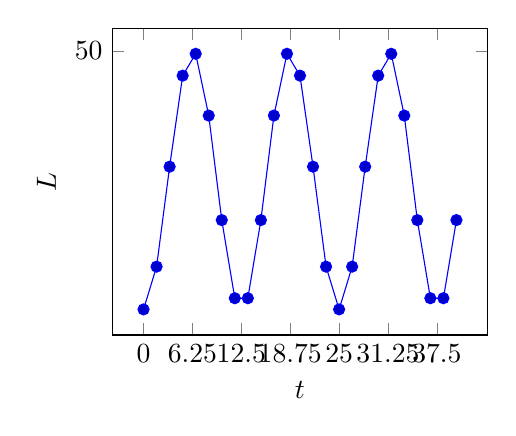
\begin{tikzpicture}
          \begin{axis}[xtick={0, 6.25, 12.5, ..., 37.5}, width=2.5in,
            ytick={50}, xlabel=$t$, ylabel=$L$] 
            \addplot+[domain=0:40] {-25*cos(deg(4*pi/25*x))+25};
          \end{axis}
        \end{tikzpicture}
      \end{center}
    \end{solution}

  \item
    \begin{problem}[\stretch{0.5}]
      Write a formula for $L(t)$.
    \end{problem}

    \begin{solution}
      It's helpful to find the amplitude, midline value, and period.  The
      time between high and low tides (6.25 hours) is half a period, so a
      whole period is 12.5 hours.  The amplitude is half of the difference
      between high tide (50) and low tide (0), so the amplitude is 25.
      The midline value is the value half-way between high tide and low
      tide, which is 25 as well.

      Based on our sketch, it makes most sense to model with a vertically
      flipped cosine function, since the function we're modeling has a
      minimum at $t = 0$.  So, the model is $L(t) = -25 \cos \left(
        \frac{2 \pi}{12.5} t \right) + 25$, which can also be written as
      $\boxed{L(t) = -25 \cos \left( \frac{4 \pi}{25} t \right) + 25}$.
    \end{solution}

  \item
    \begin{problem}[\vfill\vfill\newpage]
      At what times between $t = 0$ and $t = 12.5$ is the water level
      equal to 20 feet?  (Give all the times.)
    \end{problem}

    \begin{solution}
      We want to solve
      \begin{align*}
        -25 \cos \left( \frac{4 \pi}{25} t \right) + 25 &= 20 \\
        -25 \cos \left( \frac{4 \pi}{25} t \right) &= -5 \\
        \cos \left( \frac{4 \pi}{25} t \right) &= \frac{1}{5} \\
        \intertext{Let's substitute $u = \frac{4 \pi}{25} t$.  We're
          interested in values of $t$ in $[0, 12.5]$, which correspond to
          values of $u$ in $[0, 2 \pi]$:}
        \text{Solve } \cos u &= \frac{1}{5} \text{ for $u$ in $[0, 2 \pi]$} \\
        \intertext{We don't know any ``nice'' angles whose cosine is
          $\frac{1}{5}$, so we should express our answers in terms of
          $\arccos \left( \frac{1}{5} \right)$:} u &= \arccos \left(
          \frac{1}{5} \right), 2 \pi - \arccos \left(
          \frac{1}{5} \right) \\
        \intertext{Since $u = \frac{4 \pi}{25} t$, $t = \frac{25}{4 \pi}
          u$, so} %
        t &= \boxed{\frac{25}{4 \pi} \arccos \left( \frac{1}{5} \right),
          \frac{25}{4 \pi} \left[ 2 \pi - \arccos \left( \frac{1}{5}
            \right) \right]}
      \end{align*}
    \end{solution}

  \end{enumerate}

\item \label{fall2008-1b-midterm1-1}
  \begin{enumerate}
  \item You are traveling by elephant in the hills of northern Thailand.
    The elephant travels slowly, at a velocity of $ v(t)= \arcsin(t)$
    miles per hour where $t$ is time in hours.

    \begin{enumerate}
    \item
      \begin{problem}[1in]
        Write an integral that gives the distance you cover from $t = 0$
        to $t = 1$. 
      \end{problem}

      \begin{solution}
        Between $t = 0$ and $t = 1$, $v(t) = \arcsin t$ is positive, so
        the distance traveled is simply $\boxed{ \int_0^1 v(t)\,dt}$.
      \end{solution}

    \item

      \begin{problem}[\newpage]
        By evaluating the integral you wrote down, find the exact distance
        you cover from $t= 0$ to $t = 1$.  (\emph{Hint:} Slice!)
      \end{problem}

      \begin{solution} % solution originally written by Jameel, modified by
        % Janet
        You probably don't know an antiderivative of $\arcsin t$ off the
        top of your head (and you're not expected to!).  Instead, let's
        interpret the integral as an area and slice horizontally.  We know that
        $\displaystyle \int_0^1 \arcsin t\,dt$ can be interpreted as the
        area under the curve $y = \arcsin t$ between $t = 0$ and $t = 1$,
        which is the shaded region shown on the left:
        \begin{center}
          \begin{tikzpicture}
            \begin{axis}[xtick={1}, xlabel=$t$, ylabel=$y$, 
              ytick={1.57}, yticklabels={$\frac{\pi}{2}$}, axis
              on top, clip=false, width=2in, height=2.5in]
              \addplot+[domain=0:1, fillregion] {rad(asin(x))}
              \closedcycle; %
              \addplot+[domain=-pi/2:pi/2] ({sin(deg(x))}, x) node[above]
              {$y = \arcsin t$}; %
            \end{axis}
          \end{tikzpicture}
          \hspace{0.5in}
          \begin{tikzpicture}
            \begin{axis}[xtick={1}, xlabel=$t$, ylabel=$y$, 
              ytick={1.57, 0.9817}, yticklabels={$\frac{\pi}{2}$, $y_k$}, axis
              on top, clip=false, width=2in, height=2.5in]
              \addplot+[domain=0:1, fillregion] {rad(asin(x))}
              \closedcycle; %
              \addplot[horizslices] coordinates {(1, 0) (1, {pi/16}) (1,
                {pi/8}) (1, {(3*pi)/16}) (1, {pi/4}) (1, {(5*pi)/16}) (1,
                {(3*pi)/8}) (1, {(7*pi)/16}) (1, {pi/2}) }; %
              \addplot+[domain=0:1, fill=white, draw=none] {rad(asin(x))}
              -- (0, {pi/2}) -- (0, 0); %
              \addplot+[domain=-pi/2:pi/2] ({sin(deg(x))}, x) node[above]
              {$y = \arcsin t$}; %
              \draw[fill=cyan, draw=blue, fill opacity=0.75] (1, pi/4) --
              ({sin(deg(5*pi/16))}, pi/4) -- ({sin(deg(5*pi/16))},
              5*pi/16) -- (1, 5*pi/16) -- cycle; %
              \draw[dashed] (0, 5*pi/16) -- ({sin(deg(5*pi/16))},
              5*pi/16); %
            \end{axis}
          \end{tikzpicture}
        \end{center}
        We want to slice horizontally, which means we slice the interval
        $\left[ 0, \frac{\pi}{2} \right]$ (on the $y$-axis) into $n$ pieces,
        each of equal height $\Delta y$.  We label $y_0 = 0, \ldots, y_n =
        \frac{\pi}{2}$ as usual and focus on the $k$-th slice, as shown in
        the right picture above.

        The width of the slice is (right $t$-coordinate) $-$ (left
        $t$-coordinate); the right $t$-coordinate is 1.  The left
        $t$-coordinate is on the curve $y = \arcsin t$ (which can be
        rewritten as $t = \sin y$), so it is $\sin y_k$.  So,
        \begin{align*}
          \text{area of the $k$-th slice} & \approx \text{(width of slice)
            (height of slice)} \\
          & \approx [1-\sin(y_k)] \Delta y
        \end{align*}
        Summing over all slices and taking the limit as the number of slices
        $\to \infty$, the area of the region is 
        \begin{align*}
          \int_0^{\pi / 2} (1 - \sin y)\,dy & = y + \cos y \Big|_0^{\pi/2} \\
          & = \boxed{\frac{\pi}{2} - 1}
        \end{align*}
        So, the distance traveled is $\frac{\pi}{2} - 1$ miles. 
      \end{solution}
    \end{enumerate}

  \item 


    The elephants drink at a circular pool of water of radius 3 meters.
    The vegetation around the pool has been trampled.  The density of mud
    at a distance $x$ meters from the edge of the pool is given by
    $\rho(x)$ kg per square meter.

    \begin{enumerate}
    \item 
      \begin{problem}[\stretch{1.5}]
        Write an integral that gives the number of kilograms of mud within
        7 meters of the edge of the pool.
      \end{problem}

      \begin{solution}
        Here is a picture of the region we are interested in: 
        \begin{center}
          \begin{tikzpicture}
            \begin{axis}[xmin=3, xmax=10, ymin=-9, ymax=9, clip=false, x=0.2cm,
              y=0.2cm, hide y axis, xtick={3.01, 9}, 
              xticklabels={0, 7}]
              \draw[fill=lightgray, fill opacity=0.5] (0, 0) circle (9);
              \draw[fill=white] (0, 0) circle (3);
              \filldraw[black] (0, 0) circle(1.5pt);
              \draw (10, 0) node[right] {$x$};
              \draw (0, 0) -- node[Anchor=210, inner sep=0.5pt] {3} (120: 3);
              % \draw (0, 0) -- node[Anchor=225, inner sep=1pt] {9} (135:9);
            \end{axis}
          \end{tikzpicture}
        \end{center}
        The shaded portion is the area we need to look at; the hole in the
        middle is the pool of water.  We've also drawn an ``$x$-axis'' in
        the picture to show that $x$ measures distance from the edge of the
        pool. 

        Since the density of mud varies with distance from the edge of the
        pool, we know we will want to slice so that all points in a slice
        are (roughly) the same distance from the edge of the pool.  So,
        we'll slice into concentric rings around the pool.  This means
        we'll slice $[0, 7]$ into $n$ pieces of equal length $\Delta x$,
        and label $x_0 = 0, \ldots, x_n = 7$ as usual.  Let's focus on the
        $k$-th slice:
        \begin{center}
          \begin{tikzpicture}
            \begin{axis}[xmin=3, xmax=10, ymin=-9, ymax=9, clip=false, x=0.2cm,
              y=0.2cm, hide y axis, xtick={3, 4, ..., 9}, 
              xticklabels={,,,,$x_k$,,}, axis on top=true, tick label
              style={fill=none}] 
              \draw[fill=white!90!black] (0, 0) circle (9);
              \draw[fill=cyan] (0, 0) circle (7);
              \draw[fill=white!90!black] (0, 0) circle (6);
              \draw[fill=white] (0, 0) circle (3);
              \filldraw[black] (0, 0) circle(1.5pt);
              \draw (10, 0) node[right] {$x$};
              \draw (0, 0) -- node[Anchor=210, inner sep=0.5pt] {3} (120: 3);
              \pgfplotsforeachungrouped \x in {3, 4, ..., 9}
              {
                \edef\temp{
                  \noexpand\draw (0, 0) circle(\x);
                }
                \temp
              }              
            \end{axis}
          \end{tikzpicture}
        \end{center}
        This slice has thickness $\Delta x$, and we can approximate its
        radius as $3+x_k$.  So,
        \begin{align*}
          \text{area of $k$-th slice} & \approx (\text{circumference of
            $k$-th slice})(\text{thickness of $k$-th slice}) \\
          & \approx 2 \pi (3 + x_k) \Delta x \\
          \text{amount of mud in $k$-th slice} & \approx (\text{density of
            mud in $k$-th slice}) (\text{area of $k$-th
            slice}) \\
          & \approx \rho (x_k) \cdot 2 \pi (3 + x_k) \Delta x
        \end{align*}
        Summing over all slices and taking the limit as the number of
        slices $\to \infty$, the amount of mud within $7$ m of the edge of
        the pool is $\boxed{\int_0^{7} 2\pi(3+x) \rho(x)\,dx}$.
      \end{solution}

    \item
      \begin{problem}[\vfill\newpage]
        Evaluate your integral if $\rho(x) = \dfrac{1}{x^2 + 1}$. 
      \end{problem}

      \begin{solution}
        We are supposed to evaluate $\displaystyle \int_0^7 \frac{2 \pi (3
          + x)}{x^2 + 1}\,dx$:
        \begin{align*}
          \int_0^7 \frac{2 \pi (3 + x)}{x^2 + 1}\,dx &= 2 \pi \int_0^7
          \frac{3 + x}{x^2 + 1}\,dx \\
          &= 2 \pi \left( \int_0^7 \frac{3}{x^2 + 1}\,dx + \int_0^7
            \frac{x}{x^2 + 1}\,dx \right)
        \end{align*}
        Let's work on these two integrals separately.  For the first,
        \begin{align*}
          \int_0^7 \frac{3}{x^2 + 1}\,dx &= 3 \arctan x \Big|_0^7 \\
          &= 3 \arctan 7 - 3 \arctan 0 \\
          & = 3 \arctan 7 \text{ since $\arctan 0 = 0$}
        \end{align*}
        For the second, let's substitute $u = x^2 + 1$; then, $du =
        2x\,dx$, so $\frac{du}{2} = x\,dx$:
        \begin{align*}
          \int_0^7 \frac{\subd{x}}{\sub{x^2 + 1}}\,\subd{dx} &=
          \int_1^{50}
          \frac{1}{\sub{u}} \cdot \subd{\frac{du}{2}} \\
          &= \left. \frac{1}{2} \ln |u| \right|_1^{50} \\
          &= \frac{1}{2} \left( \ln 50 - \ln 1 \right) \\
          &= \frac{1}{2} \ln 50 \text{ since $\ln 1 = 0$}
        \end{align*}
        So, 
        \begin{align*}
          \int_0^7 \frac{2 \pi (3 + x)}{x^2 + 1}\,dx &= 
          2 \pi \left( 3 \arctan 7 + \frac{1}{2} \ln 50 \right) \\
          &= \boxed{6 \pi \arctan 7 + \pi \ln 50}
        \end{align*}
      \end{solution}

    \end{enumerate}
  \end{enumerate}

\item \label{Shanelle-optimization}


\begin{problem}
Leah is building a right triangular fence to enclose her garden. She measures that the longest side of the fence must be 12 ft wide as shown below. Find the angle $\theta$ that maximizes the length of fencing needed to surround the garden. 
\end{problem}

\begin{tikzpicture}

  % Triangle vertices
  \coordinate (A) at (3,0);
  \coordinate (B) at (0,-4); 
  \coordinate (C) at (0,0);

  % Draw the triangle
  \draw[thick] (A) -- node[midway, below right] {12 ft} (B) -- (C) -- cycle;

  % Mark the right angle at C
  \draw[thick] (C) ++(0.4,0) -- ++(0,-0.4) -- ++(-0.4,0);

  % Label angle theta at A
  \node at ($(B)+(0.2,0.6)$) {\large$\theta$};


\end{tikzpicture}

\begin{solution}
    \textbf{Goal:} Find the value of $\theta$ that maximized the length of fencing needed.

    \textbf{Given:} The longest side of the fence (the hypotenuse of the triangle) is 12 feet wide.

    Let $x$ and $y$ be the lengths of the legs of the right triangle.

\begin{tikzpicture}

  % Triangle vertices
  \coordinate (A) at (3,0);
  \coordinate (B) at (0,-4); 
  \coordinate (C) at (0,0);

  % Draw the triangle
  \draw[thick] (A) -- node[midway, below right] {12 ft} (B) -- node[midway, left] {$y$} (C) -- node[midway, above] {$x$} cycle;

  % Mark the right angle at C
  \draw[thick] (C) ++(0.4,0) -- ++(0,-0.4) -- ++(-0.4,0);

  % Label angle theta at A
  \node at ($(B)+(0.2,0.6)$) {\large$\theta$};


\end{tikzpicture}

    The length of fencing needed $L$ is given by $L=x+y+12$. We want to write $L$ as a function of $\theta$, so let's first write $x$ and $y$ in terms of $\theta$. 

    Based on the diagram we see that $\sin \theta =\dfrac{x}{12}$ and $\cos \theta = \dfrac{y}{12}$, so $x=12\sin \theta$ and $y=12\cos\theta$. 

    This gives us the following function:

    \[L(\theta)=12\sin\theta + 12\cos\theta + 12\]

    To maximize $L(\theta)$ on $\left[0,\dfrac{\pi}{2}\right]$, we want to find the critical points, so we'll start with finding $L'(\theta)$

    \[L'(\theta)=12\cos\theta - 12\sin\theta\]

    Then we'll set $L'(\theta)$ equal to $0$ and solve for $\theta$:

    \begin{align*}
        0 &= \cos\theta - 12\sin\theta\\
        12\sin\theta &= 12\cos\theta\\
        \tan\theta &= 1
    \end{align*}
    $\theta$ is an acute angle whose tangent value is $1$, so $\theta=\dfrac{\pi}{4}$. Since the domain is a closed interval, we can determine whether $\theta=\dfrac{\pi}{4}$ is a global maximum by comparing the value of the function at $\dfrac{\pi}{4}$ and the endpoints:

    \[L(0)=12\sin 0 + 12\cos 0 + 12 = 24\]
    \[L\left(\dfrac{\pi}{4}\right)=12\sin\left(\dfrac{\pi}{4}\right) + 12\cos \left(\dfrac{\pi}{4}\right) + 12 = 12\left(\dfrac{\sqrt{2}}{2}\right)+12\left(\dfrac{\sqrt{2}}{2}\right) + 12 = 12\sqrt{2} + 12\]
    \[L(0)=12\sin\left(\dfrac{\pi}{2}\right) + 12\cos\left(\dfrac{\pi}{2}\right) + 12 = 24\]

    The maximum value of $L(\theta)$ occurs when $\theta = \dfrac{\pi}{4}$, so the length of fencing needed to surround the garden is maximized when $\theta$ is $\dfrac{\pi}{4}$ radians.
\end{solution}

\probonly{\newpage}

\item \label{spring2011-1b-final-9}

  Nneka is growing cells for her research.  Nneka's cell population grows
  at a rate proportional to the population size.  Let $N(t)$ be the number
  of cells at time $t$, where $t$ is measured in days.  At time $t = 0$,
  she has 1000 cells.
  \begin{enumerate}
  \item \label{spring2011-1b-final-9-de}
    \begin{problem}[\stretch{0.5}]
      Write a differential equation and initial condition modeling the
      situation.  (Your differential equation will involve an unknown
      constant.) 
    \end{problem}

    \begin{problemonly}
      \textbf{Differential equation:}

      \pspace{0.15in}

      \textbf{Initial condition:}

      \pspace{0.15in}
    \end{problemonly}

    \begin{solution}
      We are told that the rate of population growth ($\frac{dN}{dt}$) is
      proportional to the population size ($N$), so $\boxed{\frac{dN}{dt}
        = k N}$ where $k$ is a constant.  We also have the initial
      condition $\boxed{N(0) = 1000}$.
    \end{solution}

  \item
    \begin{problem}[\vfill]
      When the cell population is $1200$, it is growing at an
      instantaneous rate of $48$ cells per day.  Use this to find the
      unknown constant in your differential equation from
      \ref{spring2011-1b-final-9-de}. 
    \end{problem}

    \begin{solution}
      We are told that, when $N = 1200$, $\frac{dN}{dt} = 48$.  We can
      plug this into the differential equation we found in
      \ref{spring2011-1b-final-9-de}:
      \begin{align*}
        \frac{dN}{dt} &= kN \\
        48 &= k (1200) \\
        k &= \frac{48}{1200} = 0.04
      \end{align*}
      So, $\boxed{\frac{dN}{dt} = 0.04 N}$. 
    \end{solution}

  \item
    \begin{problem}[\vfill]
      Write a formula for $N(t)$, the number of cells at time $t$. 
    \end{problem}

    \begin{solution}
      We know that the general solution to $\frac{dN}{dt} = 0.04 N$ is
      $N(t) = C e^{0.04 t}$ (see {the worksheet ``Introduction to Differential Equations''}).
      Then, $N(0) = C e^0 = C$, so the initial condition $N(0) = 1000$
      tells us that $C = 1000$.  Therefore, $\boxed{N(t) = 1000 e^{0.04
          t}}$.

      \begin{checkanswer}
        We can check this easily: If $N(t) = 1000 e^{0.04 t}$, then $N(0)
        = 1000$, and $\frac{dN}{dt} = (1000 e^{0.04 t}) 0.04 = 0.04 N$.
      \end{checkanswer}
    \end{solution}

  \item \label{spring2011-1b-final-9-time}
    \begin{problem}[\vfill]
      At what time will Nneka's cell population reach 1400 cells?
    \end{problem}

    \begin{solution}
      We want to solve
      \begin{align*}
        1000 e^{0.04 t} &= 1400 \\
        e^{0.04 t} &= 1.4 \\
        \shortintertext{Taking $\ln$ of both sides,}
        0.04 t &= \ln 1.4 \\
        t &= \boxed{\frac{\ln 1.4}{0.04}}
      \end{align*}
    \end{solution}

  % \item
  %   \begin{problem}[\nstretch{1.5}]
  %     Use linear approximation to give a decimal approximation for your
  %     answer to \ref{spring2011-1b-final-9-time}. 
  %   \end{problem}

  %   \begin{solution}
  %     We need to use linear approximation to approximate $\ln 1.4$.  The
  %     first step in linear approximation is to pick a function; in this
  %     case, let's use $f(x) = \ln (x)$.  Then, what we're trying to
  %     approximate is $f(1.4)$.  We'll do this by finding the line tangent
  %     to $f(x)$ at $x = 1$.  Why $1$?  Well, it's close to 1.4 (the value
  %     we actually care about), and it's convenient: we can easily evaluate
  %     $f(1)$.

  %     The slope of the line tangent to $f(x)$ at $x = 1$ is $f'(1)$.  The
  %     derivative of $f$ is $f'(x) = \frac{1}{x}$, so $f'(1) = 1$. To find
  %     the equation of a line, we need both a slope and a point, and the
  %     point we know on the tangent line is the point on $y = f(x)$ where
  %     $x = 1$.  This point has coordinates $(1, \ln (1)) = (1, 0)$.  So,
  %     the tangent line we're looking for is $y = 1 (x-1)$.

  %     This line is a good approximation for the original graph $y =
  %     \ln(x)$ for $x$ near $1$.  In other words, for $x$ near $1$, $\ln
  %     (x) \approx 1 (x-1)$.  Plugging in $x = 1.4$, $\ln ({1.4}) \approx 1
  %     (1.4-1) = 0.4$.  Therefore,
  %     \[ \frac{\ln (1.4)}{0.04} \approx \frac{0.4}{0.04} = \boxed{10}\] 
  %   \end{solution}

  \end{enumerate}

  \probonly{\newpage}

\item \label{spring2009-xb-midterm2-4-modified}

  The following is the graph of $\displaystyle f(x) = \sin \left(
    \frac{\pi x^3}{4} \right)$ on the interval $[-2, 2].$

  \begin{center}
    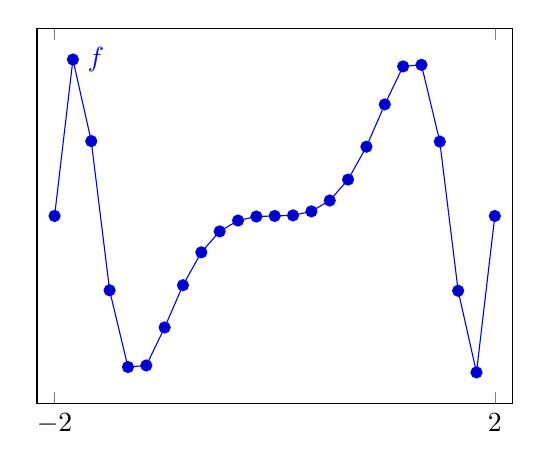
\begin{tikzpicture}
      \begin{axis}[xtick={-2, 2}, width=3in, height=2.5in, ytick=\empty,
        enlarge x limits=0.04]
        \addplot+[domain=-2:2] {sin(deg(pi*x^3/4))} node[pos=0.12,
        anchor=south west] {$f$};
      \end{axis}
    \end{tikzpicture}
  \end{center}

  \begin{enumerate}
  \item
    \begin{problem}[\vfill]
      Find the exact location of the $x$-intercepts of $f(x)$ on $[-2, 2]$.
    \end{problem}

    \begin{solution}
      We want to solve: 
      \begin{align*}
        \sin \left( \frac{\pi x^3}{4} \right) &= 0 \text{ for $x$ in }
        [-2, 2] \\
        \intertext{First, we'll substitute $u = \frac{\pi x^3}{4}$ to make
          this look simpler.  As $x$ goes from $-2$ to $2$, $\frac{\pi
            x^3}{4}$ goes from $-2 \pi$ to $2 \pi$. So, we are solving}
        \sin u &= 0 \text{ for $u$ in $[-2 \pi, 2 \pi]$} \\
        u &= - 2\pi, - \pi, 0, \pi, 2 \pi \\
        \intertext{Since $u = \frac{\pi x^3}{4}$, $x^3 = \frac{4u}{\pi}$,
          and $x = \sqrt[3]{\frac{4u}{\pi}}$.  So,} %
        x &= \boxed{-2, \sqrt[3]{-4}, 0, \sqrt[3]{4}, 2}
      \end{align*}

      \begin{checkanswer}
        It should be clear from the given diagram that $0,
        \pm 2$ are $x$-intercepts and that there are 2 more
        $x$-intercepts. 
      \end{checkanswer}
    \end{solution}

  \item
    \begin{problem}[\vfill\newpage]
      Find the exact location of the absolute minima of $f(x)$ on
      $[-2, 2]$.
    \end{problem}

    \begin{solution}
      There are two workable strategies here.  The first is our normal
      strategy for finding absolute minima: we find the critical points
      and then determine which are absolute minima.

      But here, we can actually get by without calculus, using the
      strategies we learned earlier in the semester.  In particular, the
      range of $\sin \left( \frac{\pi x^3}{4} \right)$ is $[-1, 1]$, so
      the absolute minima occur where $f(x) = -1$.  Thus, we simply need
      to solve the trig equation
      \begin{align*}
        \sin \left( \frac{\pi x^3}{4} \right) &= - 1 \text{ for $x$ in }
        [-2, 2] \\
        \intertext{As in the previous part, we'll substitute $u =
          \frac{\pi x^3}{4}$:}
        \sin u &= -1 \text{ for $u$ in $[-2\pi, 2 \pi]$} \\
        u &= - \frac{\pi}{2}, \frac{3 \pi}{2}
      \end{align*}
      Now that we've found $x$, we can go back to solve for $u$.  Since $u
      = \frac{\pi x^3}{4}$, we have $x^3 = \frac{4 u}{\pi}$, so $x =
      \sqrt[3]{ \frac{4u}{\pi} }$.  This gives us two solutions, $\boxed{
        \sqrt[3]{-2}, \sqrt[3]{6}}$.
    \end{solution}

  \end{enumerate}

  Here is the graph of $\displaystyle f(x) = \sin \left( \frac{\pi x^3}{4}
  \right)$ on $[-2, 2]$ again, now with the $x$-values of the intercepts
  and local extrema labeled.
  \begin{center}
    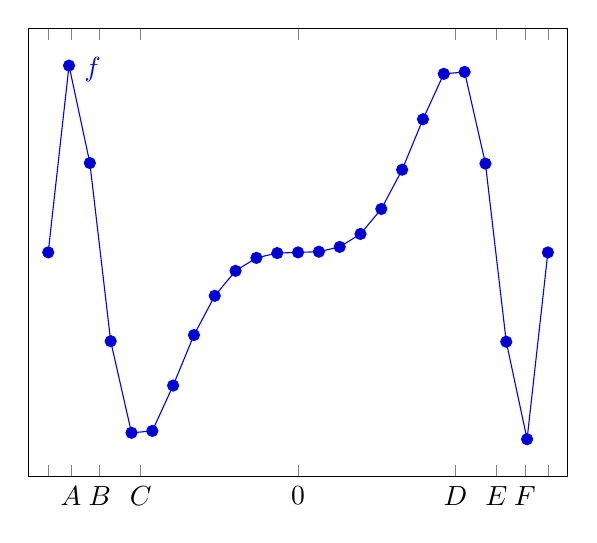
\begin{tikzpicture}
      \begin{axis}[xtick={-2, -1.81712, -1.5874, -1.25992, 0., 1.25992,
          1.5874, 1.81712, 2.}, xticklabels={, $A$, $B$, $C$, $0$, $D$,
          $E$, $F$,}, ytick=\empty, enlarge x limits=0.04]
        \addplot+[domain=-2:2] {sin(deg(pi*x^3/4))} node[pos=0.12,
        anchor=south west] {$f$};
      \end{axis}
    \end{tikzpicture}
  \end{center}
  Consider the area function $A(x) = \int_{-2}^x
  f(t)\,dt$.  For the next few parts, it is fine to give your answers in
  terms of the labeled values $A$, $B$, $C$, etc. 

  \begin{enumerate}[resume]
  \item 
    \begin{problem}[\vfill]
      For what values of $x$ in $(-2, 2)$ is $A(x)$ decreasing?
    \end{problem}

    \begin{solution}
      Our usual strategy for such a question is to make a sign chart for
      $A'$.  By FTOC 1, $A'(x)$ is equal to $f(x)$, so
      we really want to make a sign chart for $f$:
      \begin{center}
        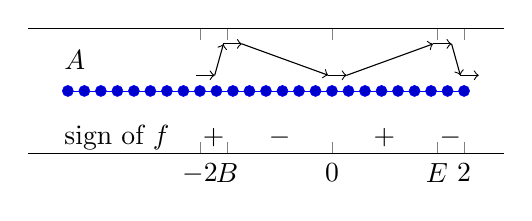
\begin{tikzpicture}
          \begin{axis}[axis y line=none, x axis line style={-},
            xtick={-2., -1.5874, 0., 1.5874, 2.}, xticklabels={$-2$, $B$,
              $0$, $E$, $2$}, ymin=-2, ymax=2, height=1.25in, width=3in,
            clip=false] 
            \addplot+[domain=-4.:2, very thin]{0}; %
            \draw (axis cs: -4.2, -1.5) node[right] {sign of $f$}; %
            \draw (axis cs: -4.2, 1) node[right] {$A$}; %
            \draw (axis cs: -1.7937, -1.5) node{$+$}; %
            \draw[->, xshift=2pt] (axis cs: -1.86, 0.5) -- (axis cs:
            -1.7274, 1.5); %
            \draw (axis cs: -0.793701, -1.5) node{$-$}; %
            \draw[->, xshift=2pt] (axis cs: -1.4474, 1.5) -- (axis cs:
            -0.14, 0.5); %
            \draw (axis cs: 0.793701, -1.5) node{$+$}; %
            \draw[->, xshift=2pt] (axis cs: 0.14, 0.5) -- (axis cs:
            1.4474, 1.5); %
            \draw (axis cs: 1.7937, -1.5) node{$-$}; %
            \draw[->, xshift=2pt] (axis cs: 1.7274, 1.5) -- (axis cs:
            1.86, 0.5); %
            \draw[->, xshift=2pt] (axis cs: -2.14, 0.5) -- (axis cs:
            -1.86, 0.5); %
            \draw[->, xshift=2pt] (axis cs: -1.7274, 1.5) -- (axis cs:
            -1.4474, 1.5); %
            \draw[->, xshift=2pt] (axis cs: -0.14, 0.5) -- (axis cs: 0.14,
            0.5); %
            \draw[->, xshift=2pt] (axis cs: 1.4474, 1.5) -- (axis cs:
            1.7274, 1.5); %
            \draw[->, xshift=2pt] (axis cs: 1.86, 0.5) -- (axis cs: 2.14,
            0.5); %
          \end{axis}
        \end{tikzpicture}
      \end{center}
      From this, we can see that $A$ is decreasing on \fbox{$(B,
        0)$ and $(E, 2)$}.

    \end{solution}

  \item
    \begin{problem}[\vfill\newpage]
      For what values of $x$ in $(-2, 2)$ is the graph of $A(x)$
      concave down?
    \end{problem}

    \begin{solution}
      $A(x)$ is concave down when $A'(x) = f(x)$ is
      decreasing, which happens on the intervals \fbox{$(A, C)$ and $(D,
        F)$}.
    \end{solution}

  \item
    \begin{problem}[\vfill]
      At what $x$-value(s) in $(-2, 2)$ does $A(x)$ have local
      maxima? 
    \end{problem}

    \begin{solution}
      From our sign chart, we can see that $A(x)$ has local
      maxima at $\boxed{x = B, E}$.
    \end{solution}

  \item 
    \begin{problem}[\vfill]
      At what $x$-value(s) in $[-2, 2]$ does $A(x)$ have an
      absolute minimum?
    \end{problem}

    \begin{solution}
      Since $[-2, 2]$ is a closed interval, $A(x)$ must have an
      absolute minimum on this interval.  From our sign chart, we see that
      the absolute minimum could be at $x= -2$, $x = 0$, or $x = 2$.  To
      decide among these, we need to decide which of $_{-2} A_f(-2)$,
      $_{-2} A_f(0)$, and $_{-2} A_f(2)$ is the smallest:
      \begin{align*}
        _{-2} A_f(-2) &= \int_{-2}^{-2} f(t)\,dt = 0 \\
        _{-2} A_f(0) &= \int_{-2}^0 f(t)\,dt \text{ is clearly negative} \\ 
        _{-2} A_f(2) &= \int_{-2}^2 f(t)\,dt = 0 \text{ by symmetry}
      \end{align*}
      So, $_{-2} A_f(0)$ is the smallest (most negative) of these three,
      and the absolute minimum of $A(x)$ occurs at $\boxed{x =
        0}$.
    \end{solution}

  \item
    \begin{problem}[\vfill\newpage]
      Sketch the graph of $A(x)$ on $[-2, 2]$ on the axes below.

      \probonly{\axes[width=4in, xmin=-2.1, xmax=2.1, xtick={-2, -1.81712,
          -1.5874, -1.25992, 0., 1.25992, 1.5874, 1.81712, 2.},
        xticklabels={$-2$, $A$, $B$, $C$, $0$, $D$, $E$, $F$, $2$}] }
    \end{problem}

    \begin{solution}
      Here is the graph.
      \begin{center}
        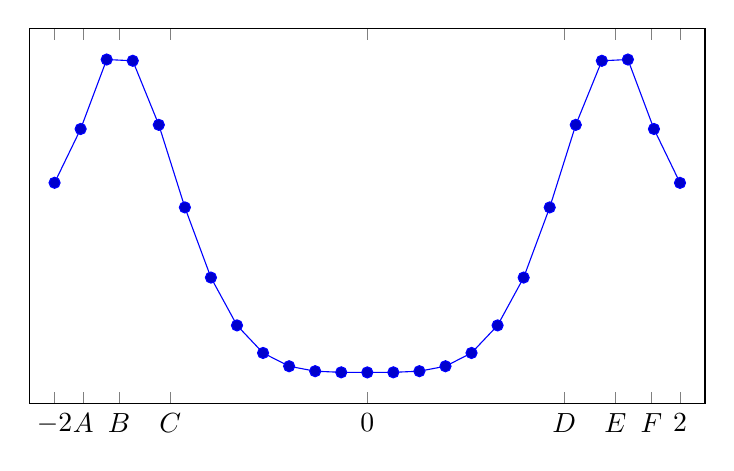
\begin{tikzpicture}
          \begin{axis}[xtick={-2, -1.81712, -1.5874, -1.25992, 0., 1.25992,
              1.5874, 1.81712, 2.}, xticklabels={$-2$, $A$, $B$, $C$, $0$, $D$,
              $E$, $F$, $2$}, ytick=\empty, enlarge x limits=0.04, width=4in,
            height=2.5in]
            \addplot+[domain=-2:2] { (pi*x^4)/16 - (pi^3*x^10)/3840 +
              (pi^5*x^16)/1966080 - (pi^7*x^22)/1816657920 +
              (pi^9*x^28)/2663550812160 - (pi^11*x^34)/5692388592844800 +
              (pi^13*x^40)/16715531679694848000 -
              (pi^15*x^46)/64588814410340892672000 - 0.3766955809953485};
          \end{axis}
        \end{tikzpicture}
      \end{center}
    \end{solution}

    \begin{grading}
      The key features your graph should have are:
      \begin{itemize}
      \item It is an even function, since the derivative $_{-2} A_f'(x) =
        f(x)$ is an odd function.
      \item It has an $x$-intercept at $x = -2$, since $_{-2} A_f(-2) =
        0$.
      \item It is increasing on $(-2, B)$, decreasing on $(B, 0)$,
        increasing on $(0, E)$, and decreasing on $(E, 2)$, with its
        absolute minimum at $x = 0$.
      \item It is concave up on $(-2, A)$, concave down on $(A, C)$,
        concave up on $(C, D)$, concave down on $(D, F)$, and concave up
        on $(F, 2)$.
      \end{itemize}
    \end{grading}
  \end{enumerate}

\item \label{riemansum-2023practice1}

\begin{problem}[\vfill]
Put the following in {\it ascending} order using ``$<$'' or ``$=$'' between each expression.  No explanation is necessary.
    \begin{enumerate}[label=\Alph*.]

    \item $\displaystyle\int_4^{10} \ln t \ dt$

    \item $\displaystyle \ln 4 + \ln 5 + \ln 6 + \ln 7 + \ln 8 + \ln 9$

    \item $\displaystyle \ln 5 + \ln 6 + \ln 7 + \ln 8 + \ln 9 + \ln 10$

    \item Zero

    \item $\displaystyle \sum_{k=1}^3 \ln (x_k) \Delta x$ where $x_k = 4 +
      k \Delta x$ and $\Delta x = 2$.

    \item $\displaystyle \sum_{k=0}^2 \ln (x_k) \Delta x$ where $x_k = 10 +
      k \Delta x$ and $\Delta x = 4$.

    \item $\displaystyle\int_4^{13} \ln t \ dt - \displaystyle\int_{10}^{13} \ln t \ dt$

    \item $\displaystyle\int_{10}^{1} \ln t \ dt$
    \end{enumerate}    
  \end{problem}

  \pspace{\newpage}

  \begin{solution} 
    Let's look at each expression:
    \begin{enumerate}[label=\Alph*.]

    \item $\displaystyle\int_4^{10} \ln t \, dt$ is the area under the
      graph of $\ln t$ between $t = 4$ and $t = 10$; here is a picture:
      \begin{center}
        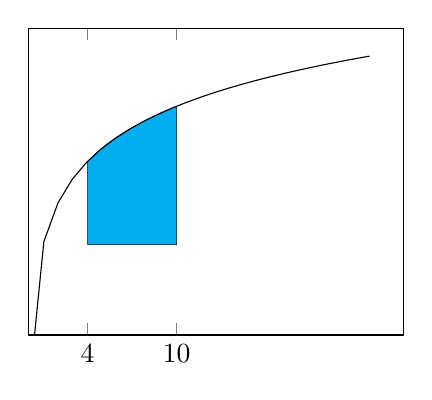
\begin{tikzpicture}
          \begin{axis}[xmin=0, ymin=-1.5, xtick={4, 10}, ytick=\empty,
            width=2.5in, cycle list=black] 
            \addplot+[domain=4:10, very thin, fill=cyan]{ln x} \closedcycle;
            \addplot+[domain=0.1:23]{ln x};
          \end{axis}
        \end{tikzpicture}
      \end{center}

    \item $\displaystyle \ln 4 + \ln 5 + \ln 6 + \ln 7 + \ln 8 + \ln 9$ is
      the left-hand estimate $L_6$ for $\displaystyle \int_4^{10} \ln
      t\,dt$.  (If we use 6 rectangles, each rectangle is 1 unit wide.)
      You can see from the graph that this is a bit less than the actual
      value of $\displaystyle \int_4^{10} \ln t\,dt$, so $B < A$.

    \item $\displaystyle \ln 5 + \ln 6 + \ln 7 + \ln 8 + \ln 9 + \ln 10$
      is the right-hand estimate $R_6$ for $\displaystyle \int_4^{10} \ln
      t\,dt$; this is a bit bigger than the actual value of $\displaystyle
      \int_4^{10} \ln t\,dt$, so $B < A < C$.

    \item All three of the previous quantities were positive, so $D < B <
      A < C$. 

    \item The notation $\displaystyle \sum_{k=1}^3 \ln (x_k) \Delta x$
      means exactly $\ln(x_1) \Delta x + \ln(x_2) \Delta x + \ln(x_3)
      \Delta x$.  The formulas $x_k = 4 + k \Delta x$ and $\Delta x = 2$
      tell us that
      \begin{align*}
        x_0 &= 4  \\
        x_1 &= 4 + \Delta x = 4 + 2 = 6 \\
        x_2 &= 4 + 2 \Delta x = 4 + 4 = 8 \\
        x_3 &= 4 + 3 \Delta x = 4 + 6 = 10
      \end{align*}
      Then, $\ln(x_1) \Delta x + \ln(x_2) \Delta x + \ln(x_3) \Delta x$ is
      exactly the area in the blue rectangles below:
      \begin{center}
        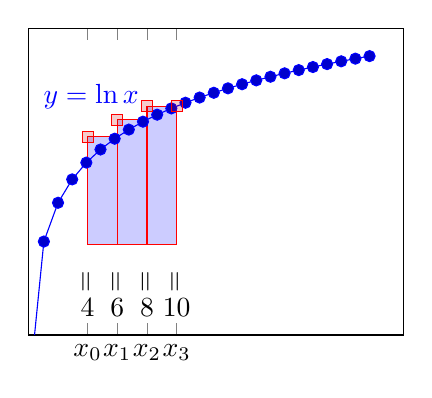
\begin{tikzpicture}
          \begin{axis}[xmin=0, ymin=-1.5, ytick=\empty, xtick={4, 6, 8, 10},
            xticklabels={$x_0$, $x_1$, $x_2$, $x_3$}, width=2.5in]            
            \addplot+[domain=0.1:23] {ln(x)} node[pos=0.4, anchor=south
            east]{$y = \ln x$};            
            \addplot+[ybar interval, fill=blue, fill opacity=0.2] plot
            coordinates
            {
              (4, {ln(6)})
              (6, {ln(8)})
              (8, {ln(10)})
              (10, {ln(10)})
            };
            \draw (axis cs: 4, 0) node[below, yshift=-6pt]
            {$\rotatebox{90}{=}$};
            \draw (axis cs: 4, 0) node[below, yshift=-16pt] {4};
            \draw (axis cs: 6, 0) node[below, yshift=-6pt]
            {$\rotatebox{90}{=}$};
            \draw (axis cs: 6, 0) node[below, yshift=-16pt] {6};
            \draw (axis cs: 8, 0) node[below, yshift=-6pt]
            {$\rotatebox{90}{=}$};
            \draw (axis cs: 8, 0) node[below, yshift=-16pt] {8};
            \draw (axis cs: 10, 0) node[below, yshift=-6pt]
            {$\rotatebox{90}{=}$};
            \draw (axis cs: 10, 0) node[below, yshift=-16pt] {10};
          \end{axis}
        \end{tikzpicture}
      \end{center}      
      So, the sum we're looking at is the right-hand sum with 3 rectangles
      that approximates $\displaystyle \int_4^{10} \ln t\,dt$.  This is an
      overestimate for $\displaystyle \int_4^{10} \ln t\,dt$, and it is a
      worse approximation than $R_6$, so it is even further off from
      $\displaystyle \int_4^{10} \ln t\,dt$ than $R_6$ was.  Therefore, $D
      < B < A < C < E$.

    \item The notation $\displaystyle \sum_{k=0}^2 \ln (x_k) \Delta x$
      means $\ln(x_0) \Delta x + \ln (x_1) \Delta x + \ln(x_2) \Delta x$.
      The formulas $x_k = 10 +
      k \Delta x$ and $\Delta x = 4$ tell us that
      \begin{align*}
        x_0 &= 10 \\
        x_1 &= 10 + \Delta x = 10 + 4 = 14 \\
        x_2 &= 10 + 2 \Delta x = 10 + 8 = 18 \\
        x_3 &= 10 + 3 \Delta x = 10 + 12 = 22
      \end{align*}
      Then, $\ln(x_0) \Delta x + \ln (x_1) \Delta x + \ln(x_2) \Delta x$
      is the area in the blue rectangles below:
      \begin{center}
        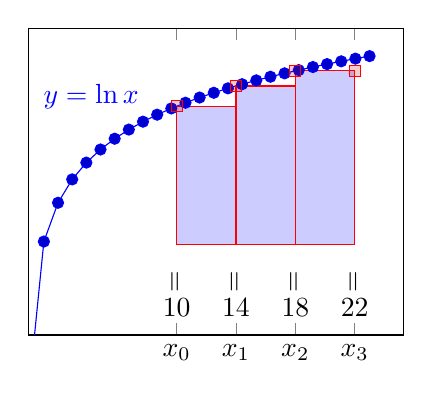
\begin{tikzpicture}
          \begin{axis}[xmin=0, ymin=-1.5, ytick=\empty, xtick={10, 14, 18,
              22}, xticklabels={$x_0$, $x_1$, $x_2$, $x_3$}, width=2.5in]
            \addplot+[domain=0.1:23] {ln(x)} node[pos=0.4, anchor=south
            east]{$y = \ln x$};            
            \addplot+[ybar interval, fill=blue, fill opacity=0.2] plot
            coordinates
            {
              (10, {ln(10)})
              (14, {ln(14)})
              (18, {ln(18)})
              (22, {ln(18)})
            };
            \pgfplotsinvokeforeach {10, 14, 18, 22}
            {
              \draw (axis cs: #1, 0) node[below, yshift=-6pt]
              {$\rotatebox{90}{=}$};
              \draw (axis cs: #1, 0) node[below, yshift=-16pt] {#1};
            }
          \end{axis}
        \end{tikzpicture}        
      \end{center}
      The area in these rectangles is clearly bigger than the area in E
      (the rectangles are both taller and wider than those in E),
      so $D < B < A < C < E < F$.

      \item We can use integral properties to rewrite $\displaystyle\int_4^{13} \ln t \ dt - \displaystyle\int_{10}^{13} \ln t \ dt$:
      \[\displaystyle\int_4^{13} \ln t \ dt - \displaystyle\int_{10}^{13} \ln t \ dt = \displaystyle\int_4^{13} \ln t \ dt + \displaystyle\int_{13}^{10} \ln t \ dt = \displaystyle\int_4^{10} \ln t \ dt\]

      This is equal to the expression in A, so $D < B < A =G < C < E  < F$.

      \item $\displaystyle\int_{10}^{1} \ln t \ dt = -\displaystyle\int_1^{10} \ln t \ dt$. We can visualize $\displaystyle\int_1^{10} \ln t \ dt$ signed area under the graph of $\ln t$ between $t=1$ and $t=10$, pictured below:

      \begin{center}
        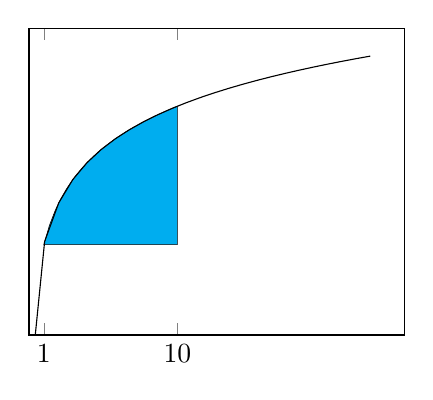
\begin{tikzpicture}
          \begin{axis}[xmin=0, ymin=-1.5, xtick={1, 10}, ytick=\empty,
            width=2.5in, cycle list=black] 
            \addplot+[domain=1:10, very thin, fill=cyan]{ln x} \closedcycle;
            \addplot+[domain=0.1:23]{ln x};
          \end{axis}
        \end{tikzpicture}
      \end{center}

        Because the area pictured is positive, $\displaystyle\int_{10}^{1} \ln t \ dt$ must be negative, so $H < D$.

    \end{enumerate}

    So, our final answer is $\boxed{H< D < B < A = G < C < E < F}$.
  \end{solution}

  \item 
  \label{spring2006-midterm1-related-rates}
  
  \begin{problem}[\newpage]
    Gladys Kravitz is convinced that her neighbor is a witch, and this
    time she's going to get proof.  She takes a 10-foot ladder over to her
    neighbor's house, where she plans to look through a window and take
    the photo which will prove that her neighbor is really a witch.

    Gladys is perched precariously at the top of a 10-foot ladder leaning
    against the back wall of her neighbor's house. Her husband, Abner,
    sees what she is up to and comes over to try to stop her. The ladder
    starts to slide down the wall. Abner is standing on the ground 6 feet
    away from the wall (behind Gladys). When the base of the ladder hits
    Abner, the top of the ladder is sliding down the wall at a rate of 4
    feet per second. How quickly is the base of the ladder moving when it
    hits Abner?

      \begin{tikzpicture}[x=0.35cm,y=0.35cm]
        \draw (-1, 0) -- (10, 0);
        \draw (2, 0) -- (6, 7);
        \draw (6, 0) -- (6, 10) -- (10, 10) -- (10, 0);
        \draw (5.5, 10) -- (8, 11) -- (10.5, 10) -- (5.5, 10);
        % \node[anchor=south, transform canvas={xshift=-2.5mm,yshift=-4.5mm}] (gladys) at (6,7);
        % {\includegraphics[width=0.5cm]{images/paro_AL_fighting}};
        % \node[anchor=south, transform canvas={yshift=-2mm}] (abner) at (0,0);
        % {\includegraphics[width=0.5cm]{images/paro_AL_hands_up}};
        \draw (0, -1) -- (6, -1);
        \draw (0, -.8) -- (0, -1.2);
        \draw (6, -.8) -- (6, -1.2);
        \draw (3, -1) node[anchor=north] {$6$ feet};
      \end{tikzpicture}      
  \end{problem}

  \begin{solution}
    \ideas{As usual, let's start by drawing two pictures, a generic
      picture that applies at any time, and a ``snapshot'' showing the
      situation at the time we care about.  We'll also label some
      variables in the generic picture.} 

    \begin{center}
      \begin{tabular}{ccc}
        \emph{Generic} & \hspace{0.25in} & \emph{Snapshot} \\
        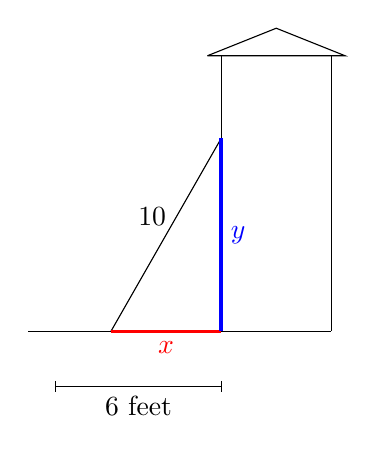
\begin{tikzpicture}[x=0.35cm,y=0.35cm]
          \draw (-1, 0) -- (10, 0);
          \draw (2, 0) -- (6, 7);
          \draw (6, 0) -- (6, 10) -- (10, 10) -- (10, 0);
          \draw (5.5, 10) -- (8, 11) -- (10.5, 10) -- (5.5, 10);
          % \node[anchor=south, transform canvas={xshift=-2.5mm,yshift=-4.5mm}] (gladys) at (6,7)
          % {\includegraphics[width=0.5cm]{images/clipart/paro_AL_fighting}};
          % \node[anchor=south, transform canvas={yshift=-2mm}] (abner) at (0,0)
          % {\includegraphics[width=0.5cm]{images/clipart/paro_AL_hands_up}};
          \draw[color=red, very thick] (2, 0) -- (6, 0);
          \draw[color=red] (4, 0) node[below] {$x$};
          \draw[color=blue, very thick] (6, 0) -- (6, 7);
          \draw[color=blue] (6, 3.5) node[anchor=west] {$y$};
          \draw (0, -2) -- (6, -2);
          \draw (0, -1.8) -- (0, -2.2);
          \draw (6, -1.8) -- (6, -2.2);
          \draw (3, -2) node[below] {$6$ feet};
          \draw (3.5, 3.5) node[anchor=south] {$10$};
        \end{tikzpicture} & & 
        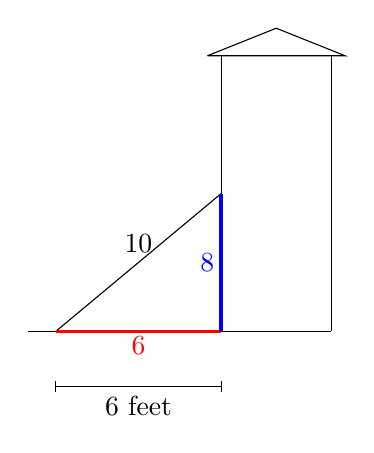
\begin{tikzpicture}[x=0.35cm,y=0.35cm]
          \draw (-1, 0) -- (10, 0);
          \draw (0, 0) -- (6, 5);
          \draw (6, 0) -- (6, 10) -- (10, 10) -- (10, 0);
          \draw (5.5, 10) -- (8, 11) -- (10.5, 10) -- (5.5, 10);
          \draw[color=red, very thick] (0, 0) -- node[midway,
          yshift=-0.5em]{$6$} (6, 0);
          \draw[color=blue, very thick] (6, 0) -- node[midway,
          xshift=-0.5em]{$8$} (6, 5);
          \draw (0, -2) -- (6, -2);
          \draw (0, -1.8) -- (0, -2.2);
          \draw (6, -1.8) -- (6, -2.2);
          \draw (3, -2) node[anchor=north] {$6$ feet};
          \draw (3, 2.5) node[anchor=south] {$10$};
          % \node[anchor=south, transform canvas={xshift=-2.5mm,yshift=-4.5mm}] (gladys) at (6,5)
          % {\includegraphics[width=0.5cm]{images/clipart/paro_AL_fighting}};
          % \node[anchor=south, transform canvas={yshift=-2mm}] (abner) at (0,0)
          % {\includegraphics[width=0.5cm]{images/clipart/paro_AL_hands_up}};
        \end{tikzpicture} 
      \end{tabular}
    \end{center}
    In the snapshot, we used the Pythagorean Theorem to figure out that
    the height is 8.

    \ideas{Next, we figure out what we know and what we want to know.}

    \highlight{
      \textbf{What we know:} At the instant we care about, $x = 6$ and
      $\dfrac{dy}{dt} = -4$ (note that this is negative because $y$ is
      decreasing). 

      \textbf{What we want to know:} $\dfrac{dx}{dt}$
    }

    \ideas{Now, we try to relate variables.  In this case, since the rate
      we know about is $\frac{d\bm{y}}{dt}$ and the rate we want to know
      is $\frac{d\bm{x}}{dt}$, we try to relate $x$ and $y$.}

    To relate variables, we use the fact that the ladder always has length
    10:

    \highlight{\textbf{Equation relating our variables:} $x^2 + y^2 = 10^2$} 

    \ideas{Once we have our relating equation, we differentiate it.  Since
      we are looking for $\frac{dx}{d\bm{t}}$, we should differentiate it
      with respect to $t$.}
    \begin{align*}
      \frac{d}{dt} (x^2 + y^2) &= \frac{d}{dt} (10^2) \\
      2x \frac{dx}{dt} + 2y \frac{dy}{dt} &= 0 \\
      \intertext{We can simplify this slightly by dividing by 2:}
      x \frac{dx}{dt} + y \frac{dy}{dt} &= 0 \\
      \intertext{Now, we can fill in the information at the time we care
        about:}
      6 \frac{dx}{dt} + (8) (-4) &= 0 \\
      6 \frac{dx}{dt} &= 32 \\
      \frac{dx}{dt} &= \boxed{\frac{16}{3} \text{ ft/s}}
    \end{align*}
  \end{solution}

\end{enumerate}
\end{document} 